%%==================================================
%% chapter03.tex for SJTU Master Thesis
%% Encoding: UTF-8
%%==================================================

\chapter{混合现实眼镜下的徒手三维建模}
\label{chap:3DModel}
本章介绍本文所设计的系统的第三个部分,通过对\ref{sec:related-cur}节中的三维建模现状及双手交互设计原则总结,设计适合混合现实眼镜场景的三维建模方法。
首先从改善双手交互的三条设计原则出发,然后为了帮助用户既保留一定的自由度,又能一定程度地优化所创建的模型弥补不同人群之间绘图技能的差异,提出自由虚拟网格平面这一想法。
自由虚拟网格平面不仅可以辅助用户创作,同时也表达了一个工作空间的概念,因而可以分离正在创作和纯移动光标两种行为。
接着阐述为了减少对整体创作过程的中断,而设计的双手职责分离概念,帮助用户在切换工具途中无缝连接前后的建模过程。
最后展示了三维建模应用场景的实现。

\section{双手交互设计原则}

首先,根据\ref{sec:related-shou}节中提到的双手交互设计三项原则,本文所设计的系统根据独有的硬件环境和应用需求做了重新评估。

%\subsection{设计原则一:保持由右及左}
\begin{enumerate}
\item 保持由右及左 \hfill\\
第一条为由右及左。本文所设计的系统维持该项原则,更精确地说,维持惯用手进行精确性操作而费惯用手进行控制类对精度要求偏低的操作。

%\subsection{设计原则二:对称的移动规模}
\item 对称的移动规模 \hfill\\
第二条原本是不对称的移动规模。本文所设计的系统将左右双手的工作空间放置在同一片区域下,因而无法也不需要对移动规模进行对应处理。
特别针对基本的物体创建,并不涉及到大规模的移动操作,于是决定采用对称的移动规模设计。

%\subsection{设计原则三:右手先行}
\item 右手先行 \hfill\\
第三条原本是左手先行,而我们采用了右手先行的原则,主要是出于对特定应用环境的考虑。
当用户在三维空间内建模时,具体在什么位置进行建模只有用户开始创建物体之后才能得知。而我们的设计是由用户使用惯用手先确定建模的初始位置,即工作空间,而后用户使用同一只手立刻进行建模,也因此保证了用户可以大致估测自己的工作空间,在想要建模的时候进入该空间范围而在不想建模的时候避开工作空间。
如果维持左手先行的原则,当交换双手时,极有可能用户会丢失自己对工作空间的概念,因而导致无法自如地建模。

\end{enumerate}
\section{自由虚拟网格平面}

自由虚拟网格平面的设计由H{\"u}rst等人\upcite{TrackingBased}启发,在其工作中提到了虚拟网格平面。
但该虚拟网格平面依附所建模物体的表面而形成,于是对于用户想要的斜面或弧度是有限制的,同样限制的还有网格的大小,于是用户只能建模一种颗粒度的物体,影响了模型的多样性。
并且由于通过移动设备(手机)才能看到建模结果,手眼之间的一致性困扰了用户的观察和理解。
同时在建模过程中,每次切换工具都会打断建模过程,非常不友好。
于是本文所设计的系统在虚拟网格平面的设计上增加了更多的自由度与操作性,提出了自由虚拟网格平面。
自由虚拟网格平面可以由用户控制它的网格大小与网格朝向,弥补前人工作的不足。

\subsection{待解决的问题}

创建物体用例有两个难点需要考虑,首先是给与用户足够的自由度进行绘制,这也是我们放弃导入模型以及使用预定义组件的原因,仅仅让用户用自己的双手进行绘制。
另一个难点是如何优化用户绘制的结果。整个应用是面向各色人群的,所以大家的绘制水平差别很大,而保证一定的绘制结果质量则是本应用设计的特色之一。
于是我们需要约束用户的绘制。
除此之外如何区分是否处在点击的状态也将在这个设计中说明。

\subsection{解决方案}

\begin{figure}[!htp]
  \centering
  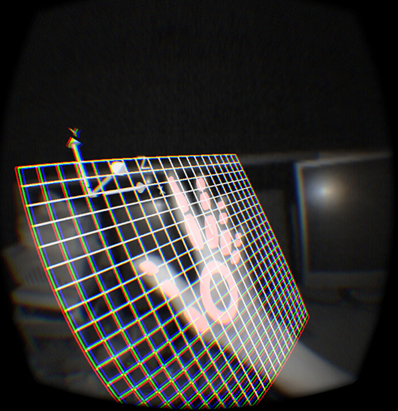
\includegraphics[width=0.4\textwidth]{chap5/fvg-show}
  \hspace{1em}
  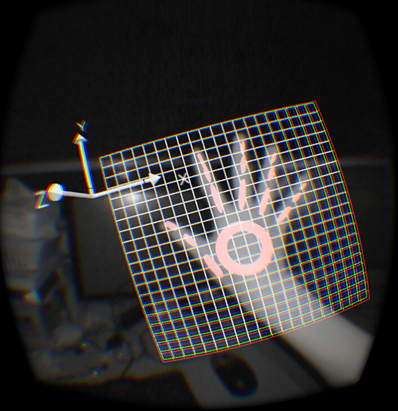
\includegraphics[width=0.4\textwidth]{chap5/fvg-show2}
  \bicaption[fig:FreeVirtualGrid]{自由虚拟网格平面}{自由虚拟网格平面}{Fig.}{Free Virtual Gird}
\end{figure}

利用辅助网格进行建模其实在各桌面建模软件中屡见不鲜,通过此类标尺一样的物体进行规范化设计的想法也深入人心。然而这样的辅助网格是否在混合现实眼镜的环境下适用得当仍未可知。因此本文所设计的系统将在此处设计一个自由的虚拟网格平面用于辅助混合现实眼镜下的三维建模。

首先,如何确定该网格平面。其创建方法如图\ref{fig:FreeVirtualGrid}所示,用户将右手自然张开伸直手指显示在眼镜前方,眼镜判断手指与掌心是否出现在同一个平面内,然后根据手掌的位置与朝向决定整个自由虚拟网格平面的位置与朝向。这个初始化操作只有在本文系统最开始运行的时候才能进行,一旦用户的手掌脱离了一个平面的约束,该网格平面便不会在随之而变动,之后也不会随用户控制变化,只会在创建模型相关的控制命令下变动。从图\ref{fig:FreeVirtualGrid}可以看到用户可以保持召唤姿势对该网格平面进行调整直到将其放置在一个合适的位置与角度下,而后所有的操控都将在这个工作环境内进行。

接下来,确定了网格平面后,该网格平面有以下两种模式供用户进行整个建模工作:涂鸦模式和拉伸模式。

%\begin{itemize}
%\item 涂鸦模式
\subsection{涂鸦模式}
\label{sec:drawMode}

\begin{figure}[!htp]
	\centering
	\subfigure{\label{fig:sketchMode}}\addtocounter{subfigure}{-2}
	\subfigure[Sketch mode in Free Virtual Gird]{\subfigure[自由虚拟网格设计中的涂鸦模式]
		{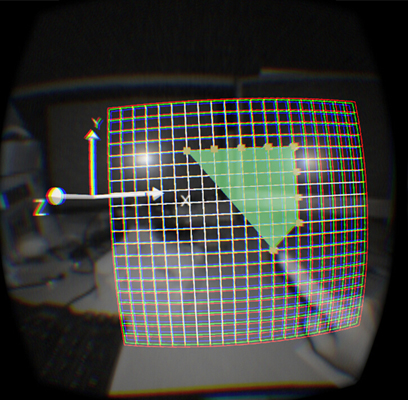
\includegraphics[height=0.25\textheight]{chap5/fvg-draw}}}
	%\vspace{-1em}
	\subfigure{\label{fig:extrudeMode}}\addtocounter{subfigure}{-2}
	\subfigure[Extrude mode in Free Virtual Gird]{\subfigure[自由虚拟网格设计中的拉伸模式]
		{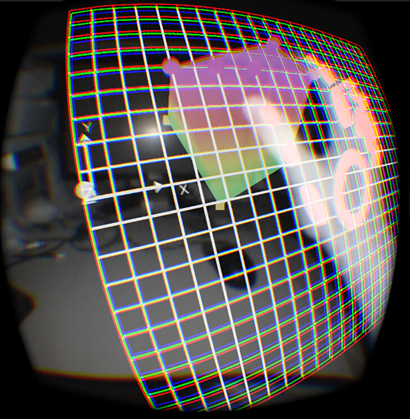
\includegraphics[height=0.25\textheight]{chap5/fvg-extrude}}}
	\bicaption[fig:mode]{自由虚拟网格设计中的绘制与拉伸模式}{自由虚拟网格设计中的绘制与拉伸模式}{Fig.}{Sketch mode and extrude mode in Free Virtual Gird}
\end{figure}

%\begin{figure}[!htp]
  %\centering
  %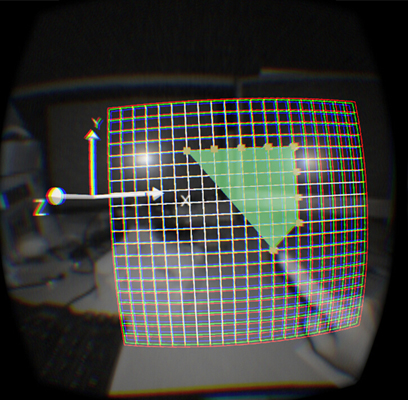
\includegraphics[width=0.5\textwidth]{chap5/fvg-draw.jpg}
  %\hspace{1em}
  %\includegraphics[width=0.3\textwidth]{chap5/testjpg}
  %\bicaption[fig:sketchMode]{自由虚拟网格设计中的涂鸦模式}{自由虚拟网格设计中的涂鸦模式}{Fig.}{Sketch mode in Free Virtual Gird}
%\end{figure}

涂鸦模式用于让用户绘制控制点。
用户伸出一根食指触发该模式。
涂鸦模式下,用户可以在自由虚拟网格平面上绘制他想要的二维图形,而本文系统会根据用户的指尖位置和该网格平面的所有交叉点进行计算。
如图\ref{fig:sketchMode}将所示,用户所有的绘制点都对齐到该网格平面的交叉点上,于是用户可以通过该设计简单轻松地进行直线,矩形等图元的绘制,而这也是保证用户绘制质量的重要因素。
如果指尖距离网格平面太远,则视为非工作空间的操控,将不会发生任何变化。
如公式\ref{eq:drawPoint}表示的一样,对用户发出指令的点进行X轴的比较,判断是哪个控制点,同理公式\ref{eq:drawPoint2}判断Y轴的情况,然后如果Z轴方向相去甚远则视为工作空间外的干扰因素,如公式\ref{eq:drawPoint3}所计算的一样。
自由虚拟网格平面将整个空间分成了三个部分,工作环境和被分开的另两个区域
也就是凭借这一点,用户可以将之前提到的移动操作和拖拽操作区分开。

\begin{equation}
\label{eq:drawPoint}
|pos_x - crossPos_x| < 0.3
\end{equation}
\begin{equation}
\label{eq:drawPoint2}
|pos_y - crossPos_y| < 0.3
\end{equation}
\begin{equation}
\label{eq:drawPoint3}
|pos_z - virtualPlane| < 1
\end{equation}

%\item 拉伸模式
\subsection{拉伸模式}
\label{sec:extrudeMode}

%\begin{figure}[!htp]
  %\centering
  %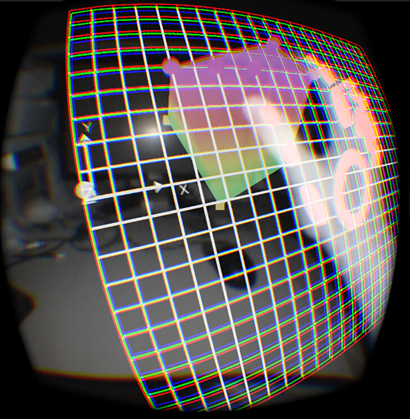
\includegraphics[width=0.5\textwidth]{chap5/fvg-extrude}
  %\hspace{1em}
  %\includegraphics[width=0.3\textwidth]{chap5/testjpg}
  %\bicaption[fig:extrudeMode]{自由虚拟网格设计中的绘拉伸模式}{自由虚拟网格设计中的拉伸模式}{Fig.}{Extrude mode in Free Virtual Gird}
%\end{figure}

拉伸模式用于让用户将二维图形拓展至三维物体。
用户伸出至少三根手指激活该模式。
拉伸模式下,用户可以选定所需的控制点,对原有的模型,二维或者三维,进行垂直于网格平面的拉伸。
如图\ref{fig:extrudeMode}所示,被选中的点将会在网格平面的法向方向延伸,可以正向法向也可以反向,本文系统都是支持的。除了最初的二维图形绘制外,一旦物体被拉伸后,就将一直作为一个三维模型存在,用户可以继续建模。
不断重复涂鸦模式和拉伸模式可以创建出复杂的模型来。

除了基本的操作以外,本文所设计的系统提出的自由虚拟网格平面可以在最开始的初始化之后调整自身的配置,这也就是它被命名为“自由”的原因。

目前支持的调整包括朝向的调整和精度的调整。

\begin{figure}[!htp]
  \centering
  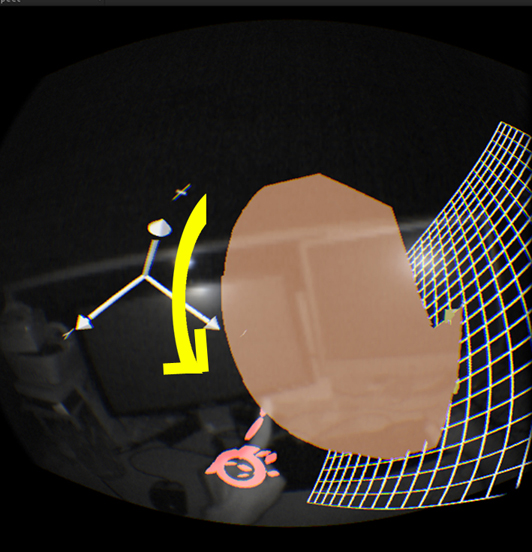
\includegraphics[width=0.4\textwidth]{chap5/fvg-rotate1}
  \hspace{1em}
  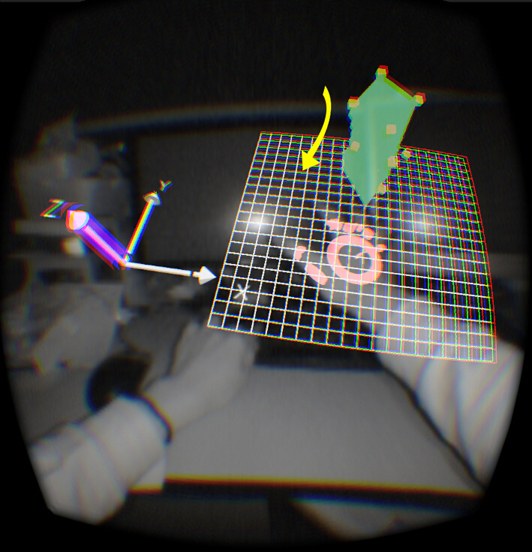
\includegraphics[width=0.4\textwidth]{chap5/fvg-rotate2}
  \bicaption[fig:rotation]{自由虚拟网格设计中的朝向调整}{自由虚拟网格设计中的朝向调整}{Fig.}{Rotation in Free Virtual Gird}
\end{figure}

\subsubsection{朝向调整}
%\begin{description}
%\item[朝向调整]\hfill\\
自由虚拟网格平面的设定是拉伸只能沿该网格平面的法向量,因而在用户进行拉伸操作时,旋转该网格平面可以使用户的拉伸方向同时得到调整,于是可以更轻松简单地创建弯折的物体。比如拱桥,比如埃菲尔铁塔。
如图\ref{fig:rotation}所示,可以看到旋转过后自由虚拟网格平面带来了模型的弯曲。

%\textbf{旋转过后的控制点如何计算的公式过程}

\begin{figure}[!htp]
  \centering
  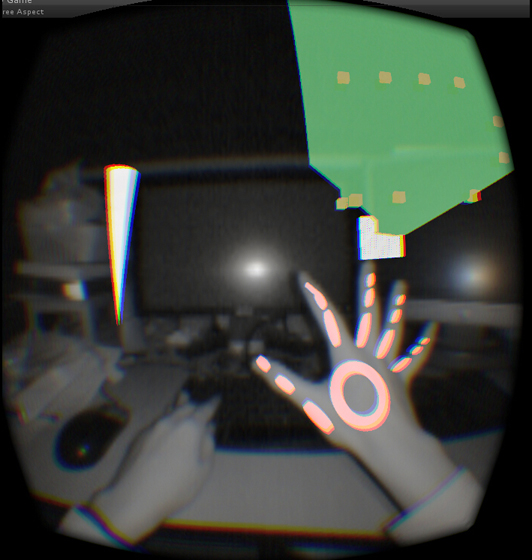
\includegraphics[width=0.4\textwidth]{chap5/fvg-scale1}
  \hspace{1em}
  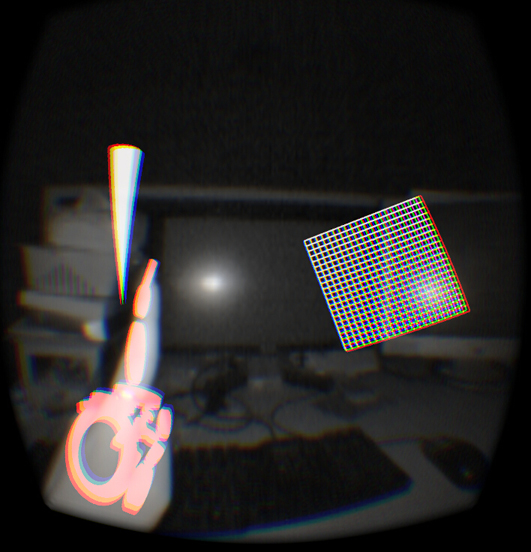
\includegraphics[width=0.4\textwidth]{chap5/fvg-scale2}
  \bicaption[fig:scalescale]{自由虚拟网格设计中的精度调整}{自由虚拟网格设计中的精度调整}{Fig.}{Scale in Free Virtual Gird}
\end{figure}

\subsubsection{精度调整}
%\item[精度调整]\hfill\\
除此之外自由虚拟网格平面在初始化之后仍旧可以调整网格的每个单元大小,所以模型的精度也可以在创建过程中变化。于是创建原型也变得可能,而有些粗颗粒度的物体则可以更简单的绘制而不需要用户对每个过程点进行劳心。
如图\ref{fig:scalescale}所示,可以看到一个棱台一样形状的物体,同样建模软件如3DMAX进行绘制,必须在选中绘制棱台的命令下才可以从底座开始绘制,然后高度,最后调整棱台的上台面。

%\end{description}

\section{职责分离的双手}

本文所设计的系统设计职责分离的双手首先为了体现混合现实眼镜的优势,该设备释放双手,所以如果能使用两只手同时进行交互是非常有利的,并且两只手完成的任务不一样,有协作有并发更可以体现该系统的高效。
另一点也是考虑到惯用手和非惯用手本就不该是一样的设计,如果将不同的职责分派下去是否会有更好的效果,这点也将在之后的评估着重讨论。

\subsection{待解决的问题}

对于专业建模软件不易于使用的一个原因是庞大的操作数量令人眼花缭乱,经常只是看着工具栏就已迷失。而另一个原因则是每次用户需要切换工具或其他命令时,必须要中断当前的建模过程,去工具栏中寻找合适的指令,而每次用户将注意力转移到工具栏或菜单栏后,整个建模的用户体验就已经被影响了。就如同\ref{sec:related-zhuangtai}节提到的一样,如何在状态切换的同时保证其显见性和平滑自然地维持整个用户体验,是很重要的。

\subsection{解决方案}

为此本文系统设计了一种方法让用户在建模途中可以在不同状态间切换同时不打断建模过程。该方法主要通过给用户的惯用手和非惯用手赋予不同的职责实现。
对于标准的单手输入设备比如鼠标,用户是很难同时进行多项任务的。
而在本文系统的设计中,利用混合现实眼镜释放双手的特性,用户可以同时使用用户的两只手进行更便捷的设计,从而创建更复杂的模型。
接下来以右手为惯用手进行阐述。
本文系统将右手设定为绘制之手,顾名思义,用户将使用且仅使用这只手进行绘制,之前\ref{sec:drawMode}节和\ref{sec:extrudeMode}节提到的绘制控制点和拉伸模型都是由绘制之手进行完成的。
它的主要职责在于创造。
而左手默认作为非惯用手,在本文所设计的系统中设定为控制之手。
负责控制当前场景的状态以及切换命令,关键在于,用户无需将绘制之手移除场景而使用控制之手进行操控,左手和右手是可以同时工作的。
目前本文所设计的系统支持两种指令:旋转和放缩。

\begin{figure}[!htp]
  \centering
	\subfigure{\label{fig:ctrl:1}}\addtocounter{subfigure}{-2}
	\subfigure[Manipulation gesture of control hand sample one]{\subfigure[控制之手的操控手势示例一]
		{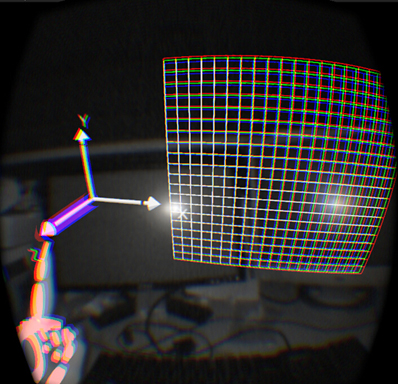
\includegraphics[height=0.25\textheight]{chap5/axis-z}}}
	\subfigure{\label{fig:ctrl:2}}\addtocounter{subfigure}{-2}
	\subfigure[Manipulation gesture of control hand sample two]{\subfigure[控制之手的操控手势示例二]
		{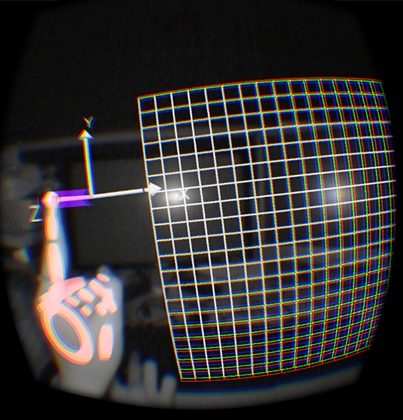
\includegraphics[height=0.25\textheight]{chap5/rotate-grab}}}
  \bicaption[fig:ctrl]{控制之手的操控手势}{控制之手的操控手势}{Fig.}{Manipulation gesture of control hand}
\end{figure}
如图\ref{fig:ctrl}所示为操控之手的控制手势,左手自然伸出一根食指,分别对旋转的工具或放缩的工具进行操作,而图\ref{fig:switch}则是对两个操控工具的切换,切换之前如图\ref{fig:switch}(a)所示为旋转工具,而切换之后如图\ref{fig:switch}(b)所示为放缩工具。扰动手腕自然旋转两圈则表示换下一个工具,这样的设计其一考虑转圈的动作可能会有误操作,所以数量上设定为两圈,其二考虑减少用户的注意力,无需用户进行特定位置的选中,任意区域只要检测到控制之手的切换手势就对工具栏进行切换。
\begin{figure}[!htp]
  \centering
  \subfigure{\label{fig:switch:1}}\addtocounter{subfigure}{-2}
	\subfigure[Rotation tool]{\subfigure[旋转工具]
		{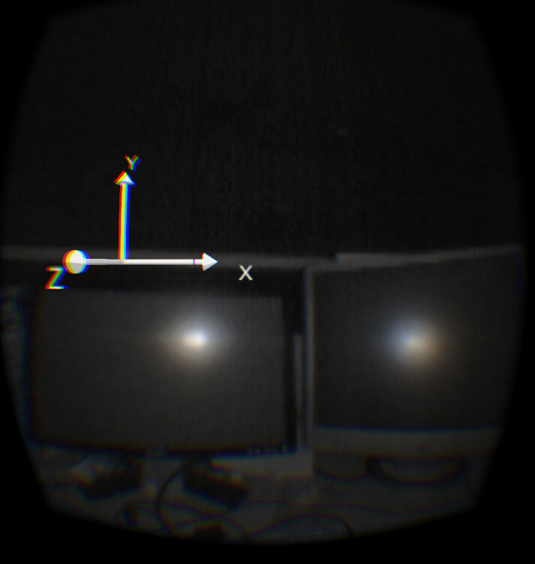
\includegraphics[width=0.3\textwidth]{chap5/axesInLeft}}}
	\subfigure{\label{fig:switch:2}}\addtocounter{subfigure}{-2}
	\subfigure[Scale tool]{\subfigure[放缩工具]
		{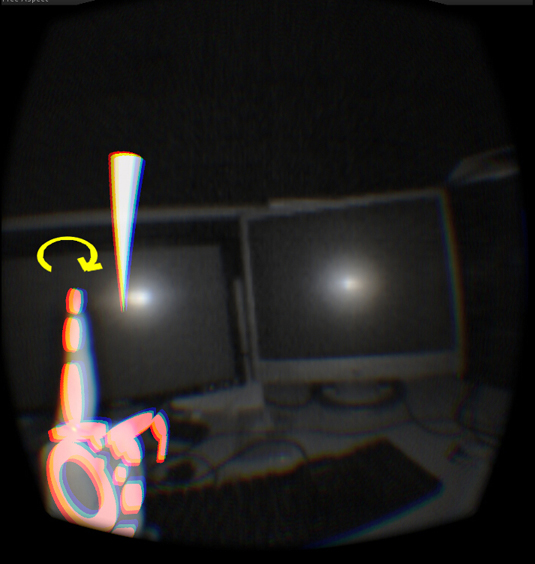
\includegraphics[width=0.3\textwidth]{chap5/scaleInLeft2}}}
  \bicaption[fig:switch]{控制之手的切换手势}{控制之手的切换手势}{Fig.}{Switch gesture of control hand}
\end{figure}

与此同时,当屏幕左方象征着工具栏的物体有了变化,如坐标轴被用户旋转后,右方的自由虚拟网格平面也会随之而旋转。
由于常见的旋转操控通常都是复杂不直观。这里本文所设计的系统采用了代理来简化旋转操作。
一共需要两步完成操作:
\begin{enumerate}[1]
\item	%\hfill \\
用户用食指抓住坐标轴中的任何一根轴的轴尖,如图\ref{fig:rotate}(a)所示
\item	%\hfill \\
用户对轴进行拖拽,坐标轴的原点不会变动,其效果和把住一个实物进行旋动的效果一致,图\ref{fig:rotate}(b)可见将X轴向上拖拽达到绕Z轴逆时针旋转的效果,可以看到图中除了坐标轴进行了这样的变化,右方的自由虚拟网格平面也进行了相同的变化。
\end{enumerate}

\begin{figure}[b]
  \centering
  \subfigure{\label{fig:rotate:1}}\addtocounter{subfigure}{-2}
	\subfigure[Before rotation]{\subfigure[旋转前]
		{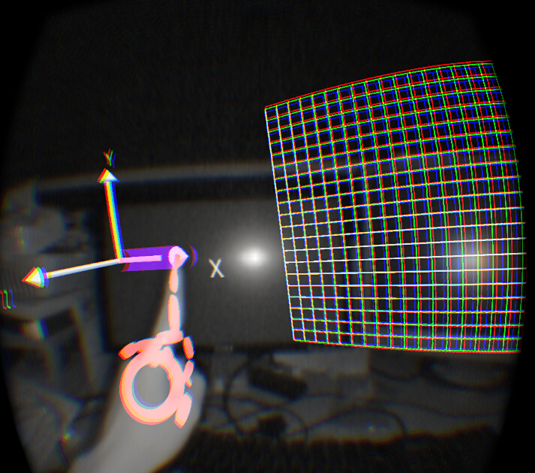
\includegraphics[height=0.25\textheight]{chap5/axis-x}}}
	\subfigure{\label{fig:rotate:2}}\addtocounter{subfigure}{-2}
	\subfigure[After rotation]{\subfigure[旋转后]
		{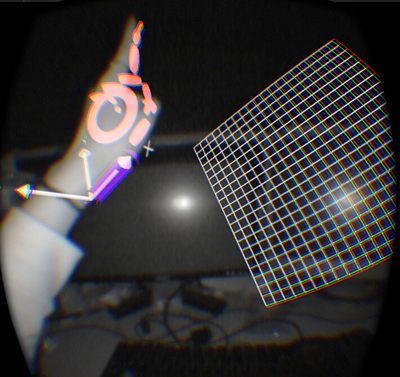
\includegraphics[height=0.25\textheight]{chap5/axis-x2}}}
  \bicaption[fig:rotate]{旋转网格平面示例}{旋转网格平面示例}{Fig.}{Rotate free virtual grid}
\end{figure}

\begin{figure}[!htp]
  \centering
   \subfigure{\label{fig:moreRotate:1}}\addtocounter{subfigure}{-2}
	\subfigure[Rotate through axis x]{\subfigure[拖拽X轴旋转]
		{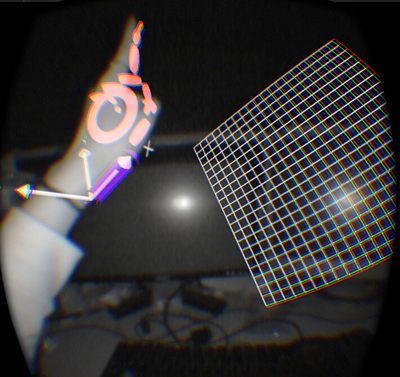
\includegraphics[height=0.18\textheight]{chap5/axis-x2}}}
	\subfigure{\label{fig:moreRotate:2}}\addtocounter{subfigure}{-2}
	\subfigure[Rotate through axis y]{\subfigure[拖拽Y轴旋转]
		{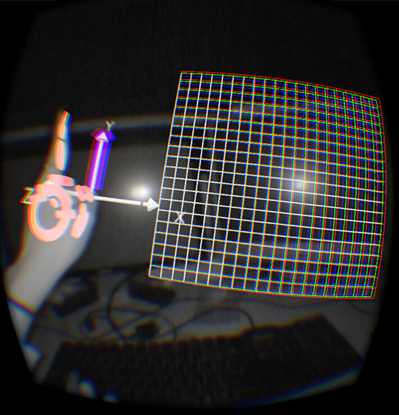
\includegraphics[height=0.18\textheight]{chap5/axis-y2}}}
		\subfigure{\label{fig:moreRotate:3}}\addtocounter{subfigure}{-2}
	\subfigure[Rotate through axis z]{\subfigure[拖拽Z轴旋转]
		{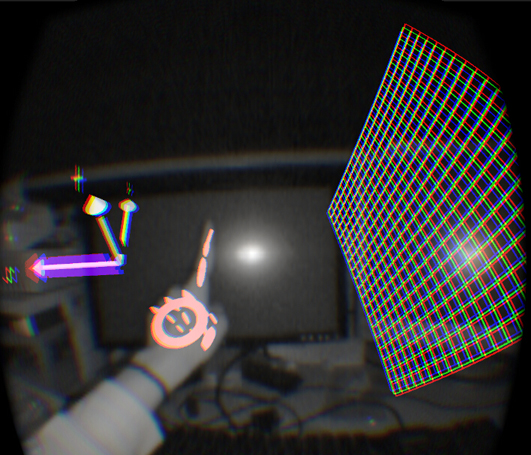
\includegraphics[height=0.18\textheight]{chap5/axis-zz2}}}
  \bicaption[fig:moreRotate]{旋转网格平面更多示例}{旋转网格平面更多示例}{Fig.}{Different types of rotation}
\end{figure}

为了更清楚地说明旋转原理,图\ref{fig:moreRotate}展示了抓住三根轴往三个标准方向旋转的事例。分别是抓住X轴上下拖拽来绕Z轴旋转(见图\ref{fig:moreRotate}(a));抓住Y轴前后拖拽来扰X轴旋转(见图\ref{fig:moreRotate}(b));和抓住Z轴左右拖拽来扰Y轴旋转(见图\ref{fig:moreRotate}(c)),坐标轴的变化和一边自由虚拟网格的变化都清晰地展示了效果。
而操控之手的旋转操作,详情见算法\ref{alg:model:rotate}:

	\begin{algorithm}  
		\caption{操控之手的旋转操作算法}  
		\label{alg:model:rotate} 
		\begin{algorithmic}  
		\REQUIRE{虚拟网格平面针对被选中的轴$Axis$和移动距离$projectLength$}
		\ENSURE{更新后的控制点$SET_c_p$}
			\STATE{将$Axis$根据$projectLength$进行旋转}
			\STATE {得到所有控制点$SET_c_p$}   
			\FOR{each $cp_c_o_o_r_d \in SET_c_p$}
				\STATE{计算世界坐标系下相对于网格平面的坐标\\$cp=cp_c_o_o_r_d*S_p_l_a_n_e*S_s_q_u_a_r_e$}
				\STATE{计算世界坐标系下的坐标\\$cp_w_o_r_l_d=transform.transformPoint(cp_w_o_r_l_d)$}
			\ENDFOR
		\end{algorithmic}  
	\end{algorithm} 

%\begin{figure}[!htp]
  %\centering
  %\includegraphics[width=0.3\textwidth]{chap5/testpng}
  %\hspace{1em}
  %\includegraphics[width=0.3\textwidth]{chap5/testjpg}
  %\bicaption[fig:scale]{缩放网格平面}{缩放网格平面}{Fig.}{Zoom in or out}
%\end{figure}

缩放手势则针对缩放工具倒圆锥进行,当用户的操控之手触及倒圆锥时,自由虚拟网格平面的单元大小就和倒圆锥上用户的手指位置绑定在了一起。用户在倒圆锥上进行上下移动会导致该网格平面变大或者变小,当用户的操控之手脱离倒圆锥时,操控自然停止,类似一个自动触发的滚动条。
	
为了保证缩放前后用户所建模型的相对位置不受变化,
\begin{algorithm}  
		\caption{操控之手的放缩操作算法}  
		\label{alg:model:scale} 
		\begin{algorithmic}  
		\REQUIRE{控制点$SET_c_p$,虚拟网格平面放缩因子$S_p_l_a_n_e$,网格大小$S_s_q_u_a_r_e$}
		\ENSURE{更新后的控制点$SET_c_p$}
			\FOR {each point $p_c_o_o_r_d \in SET_c_p$}
				\STATE{累加$p_c_o_o_r_d$求和}
				\STATE{计算世界坐标系下相对于网格平面的坐标\\$p=p_c_o_o_r_d*S_p_l_a_n_e*S_s_q_u_a_r_e$}
				\STATE{计算世界坐标系下的坐标\\$p_w_o_r_l_d=transform.transformPoint(p_w_o_r_l_d)$}
			\ENDFOR
			\STATE{平均求得中心点的坐标$pCenter_c_o_o_r_d$}
			\STATE{计算世界坐标系下相对于网格平面的坐标\\$pCenter$ 和$pCenter_o_l_d$}
			\FOR{each $p_w_o_r_l_d$}
				\STATE{将$p_w_o_r_l_d + pCenter - pCenter_n_e_w$加入控制点集合$control points$}
			\ENDFOR
		\end{algorithmic}  
\end{algorithm} 
因而系统此处默认采用中心放缩的方法,中心为用户所创建的模型在网格平面上的中心,具体算法见算法\ref{alg:model:scale}:	

\section{三维建模应用场景实现}
在设计了自由虚拟网格平面用以辅助用户绘制,及职责分离的双手原则来无缝连接建模过程中的状态切换后,接下来将描述本文系统针对的徒手三维建模场景。

\begin{figure}[!htp]
	\centering
	\subfigure{\label{fig:model:1}}\addtocounter{subfigure}{-2}
	\subfigure[House with the pinnacle]{\subfigure[尖顶房屋]
		{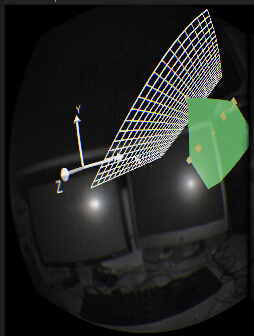
\includegraphics[height=0.3\textheight]{chap6/house}}}
	\subfigure{\label{fig:model:2}}\addtocounter{subfigure}{-2}
	\subfigure[House with flat roofs]{\subfigure[平顶房屋]
		{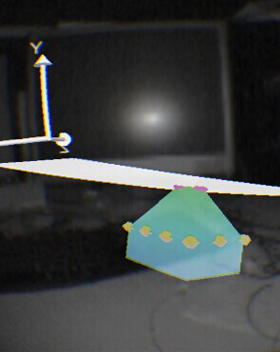
\includegraphics[height=0.3\textheight]{chap6/house-2}}}
	\bicaption[fig:model:house]{建模场景之房屋}{建模场景之房屋}{Fig.}{Houses in model application}
	\vspace{-1em}
\end{figure}

\subsection{应用简介}
徒手三维建模场景是在任意场景下,用户戴上系统配置的混合现实眼镜,不佩戴任何其他辅助工具进行双手建模的应用场景。
针对本文系统设计的三维建模特点,本应用特对设计了以下三个建模目标进行效果展示。
\begin{enumerate}
\item 基本房屋\hfill\\ 
一个基本的房屋必须有一个柱形的房屋本体,通常以方形为主,不规则多边形亦是一种选择,而后如果是一幢独立房屋则会有一个屋顶,以尖顶居多,平顶也是一种常见设计。
\item 艺术花瓶\hfill\\ 
一个艺术花瓶整体形状将呈现一个柱形,但在柱形区域的横截面通常为不同半径的圆盘,否则其将不为一个花瓶而只是一个圆柱体罢了,通过半径的调整将展现自成一脉的艺术花瓶。
\item 一座拱桥\hfill\\ 
一座拱桥的整体构架是一个半圆,或高或低的半圆皆可,而这座半圆始末为拱桥的桥墩,通常桥墩形状为长方形,其他的形状亦可。
\end{enumerate}

用户将通过以上三种建模目标感受自由虚拟网格及职责分离原则的设计。

\subsection{效果展示}

图\ref{fig:model:house}显示了一个基本房屋。用户创建了方形的底座,从图上可以看到黄色的控制点,然后向上拉伸,接着选中方形拉伸区域内靠中间的控制点,进行第二次拉伸,于是完成了图\ref{fig:model:house}(a)中所见的尖顶,如果拉伸时选中两个点将会产生平顶效果,如图\ref{fig:model:house}(b)所示。
此处建模房屋只需要使用绘制之手的涂鸦模式和拉伸模式,简单易行。

\begin{figure}[t]
  \centering
  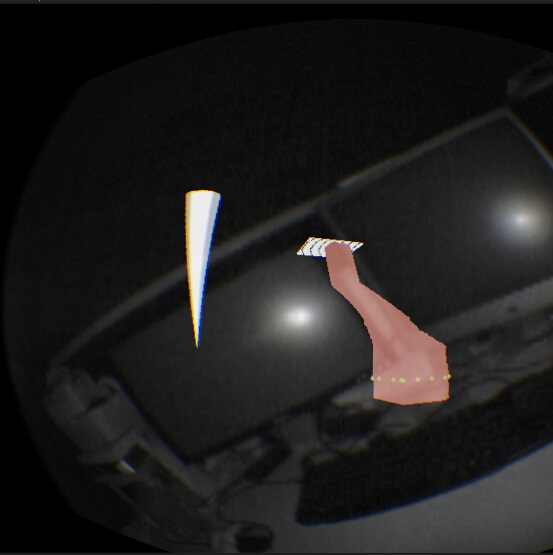
\includegraphics[width=0.4\textwidth]{chap6/vase}
  \bicaption[fig:model:vase]{建模场景之花瓶}{建模场景之花瓶}{Fig.}{Vase in model application}
\end{figure}

图\ref{fig:model:vase}显示了一个艺术花瓶。可以看到艺术花瓶最开始由底部平稳拉伸向上,而后采用控制之手切换工具调整网格大小,于是花瓶的半径开始变小,
而在调整大小的操控环境下,用户的操控之手离开倒圆锥工具,此时便无法调整半径大小,于是绘制之手又可以将花瓶平稳向上拉伸,也就是后三分之一阶段花瓶半径保持不变的功效。此处需要结合操控之手和绘制之手共同完成协作,而在工具切换时从来不需要绘制之手放下或者等待,因为建模的流程从未中断。

\begin{figure}[t]
  \centering
  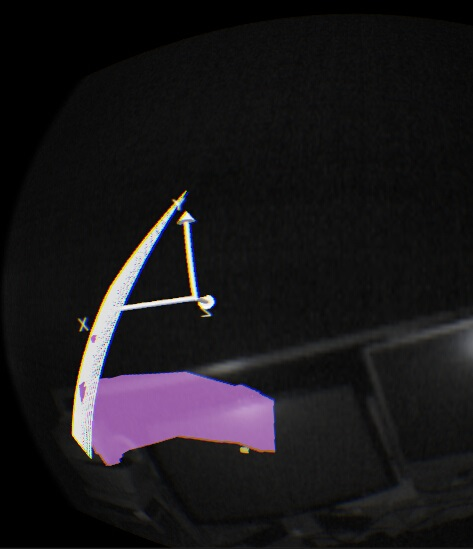
\includegraphics[width=0.4\textwidth]{chap6/bridge}
  \bicaption[fig:model:bridge]{建模场景之拱桥}{建模场景之拱桥}{Fig.}{Bridge in model application}
\end{figure}

图\ref{fig:model:bridge}显示了一座微微弯曲的拱桥。用户首先创建了一个长方形的桥墩,桥墩面积并不大,也给之后的旋转拉伸提供了空间。
而后用户将桥墩慢慢上拉,并同时用操控之手选中坐标轴工具中的Y轴,将Y轴向左拖拉,从而达到整个网格平面沿Z轴顺时针旋转的效果。
于是桥墩在向上的同时开始向右旋转,同时进行着旋转和拉伸可以看到桥墩缓缓向左方延伸。
直到最后形成一个微微弯曲的拱桥。

通过图\ref{fig:model:house}、图\ref{fig:model:vase}和\ref{fig:model:bridge}可见在重新设计的双手交互原则、自由虚拟网格的辅助及职责分离的思想支持下,用户可以简单地创作一些相对复杂的三维模型,而针对三维模型的效果、时间开销等可行性与易用性的评估将会在下章详细描述。

\section{本章小结}

本章具体介绍了混合现实眼镜下的徒手建模设计。
首先确定了本文所设计的系统采用的双手交互原则,将前人的工作和本文所设计的系统所处的硬件与应用环境结合得到适合的新原则。
然后提出本文所设计的系统对于三维建模应用的第一个新方法,自由虚拟网格平面。
与前人工作中提到的虚拟网格平面不同在于其自由度,其一为可以在初始化配置后进行朝向的旋转,其二为单元格大小的调整,于是可以支持弯曲的和精度不同的模型建设,仅是这两点就可以创建复杂的模型了。
不仅如此,自由虚拟网格平面解决了一部分的状态切换问题,通过自由虚拟网格平面的提示,用户清晰地知道自己的工作环境,因而不会有单纯的手指移动导致对模型的误操作,系统会判断当前手指是否在工作环境平面内。
接着提出了第二个辅助建模工作的方法,双手职责分离。为了突出混合现实眼镜释放双手的特性并扩大双手操作的益处,本文所设计的系统给惯用手和非惯用手安排了不一样的任务,一则负责精细具体的绘制,一则负责偏控制的命令操作。
并对其中涉及的算法都予以简单概述。
最后展示了通过以上设计展开的三维建模应用场景效果,通过基本房屋、艺术花瓶和拱桥三个建模目标体现了本文系统所设计的徒手三维建模方法能的实用性。